\documentclass[11pt,a4paper]{article}

\usepackage{Act}

\begin{document}
\input{\detokenize{/home/fenarius/Travail/Cours/cpge-info/latex/Macros.tex}}
\ModeExercice
\Colles{: session 1}{Bases du C -- Notions d'algorithmique}

\setcounter{Exercise}{0}

\begin{Exercise}[title = {nombre de chiffres d'un entier}]
\Question{Ecrire une fonction {\tt nombre\_chiffres} en C qui prend en argument un entier  supposé positif et renvoie le nombre de chiffres de cet entier dans son écriture en base 10. Par exemple {\tt nombre\_chiffres(1912)} renvoie 4.}
\Question{Dessiner le graphe de flot de contrôle de cette fonction.}
\Question{Proposer des tests afin de valider le comportement de cette fonction.}
\end{Exercise}

\begin{Exercise}[title = {chiffrement de César}]\\
    L'une des plus ancienne méthodes de chiffrement est le code de César qui consiste simplement à décaler chaque lettre d'une distance fixe dans l'alphabet. Par exemple si cette distance (appelée clé de chiffrement) est 3, la lettre $A$ devient $D$, $B$ devient $E$, et ainsi de suite. Pour les dernières lettres on reprend au début de l'alphabet. Par exemple toujours avec une distance de 3, $X$ devient $A$, $Y$ devient $B$ et $Z$ devient $C$. Ce fonctionnement est illustré ci-dessous : \medskip
\begin{center}
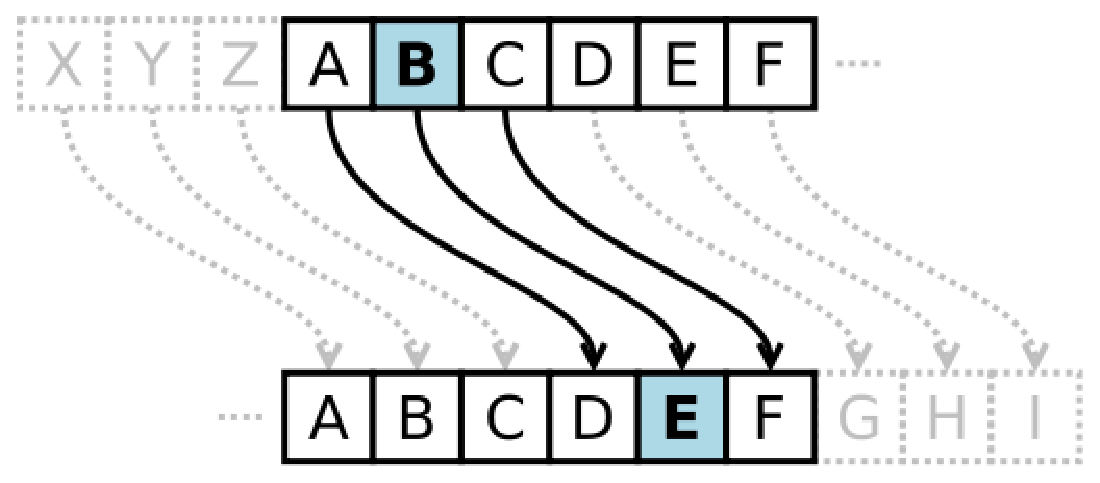
\includegraphics[width=8cm]{cesar.eps}
\end{center}
\Question{Ecrire une fonction {\tt chiffre\_lettre} qui prend en argument un caractère  {\tt car}  et un entier {\tt cle} et renvoie un le caractère {\tt car} chiffré avec le décalage {\tt cle} tel que décrit ci-dessus.\\ Par exemple {\tt chiffre\_lettre('A',3)} doit renvoyer {\tt 'D'}.}
\Question{Modifier la fonction précédente afin que seules les lettres majuscules soient chiffrées, si un autre caractère est envoyée à la fonction {\tt chiffre\_lettre} alors ce même caractère est renvoyé par la fonction. Par exemple {\tt chiffre\_lettre('!',3)} doit renvoyer {\tt '!'}.}
\end{Exercise}


\begin{Exercise}[title = {pangramme}]\\
    Un \textit{pangramme} est un phrase comportant toutes les lettres de l'alphabet, l'un des exemples les plus connus est la phrase \og{} \textit{portez ce vieux whisky au juge blond qui fume}\fg{}. 
    \Question{Ecrire une fonction {\tt est\_pangramme} qui prend en argument une chaine de caractères écrite en majuscules et renvoie {\tt true} s'il s'agit d'un pangramme et  {\tt false} sinon.}
    \Question{Proposer un jeu de test afin de valider le comportement de cette fonction.}
\end{Exercise}

\begin{Exercise}[title = {nombres narcissiques}]\\
    Un entier naturel $n$ s'écrivant avec $p$ chiffres en base 10 est dit \textit{narcissique} lorsqu'il est égal à la somme des puissances $p$ième de ses chiffres. Par exemples, :
    \begin{itemize}
    \item $153$ est un nombre narcissique car $1^3 + 5^3 + 3^3 = 153$ ($1 + 125 + 27$),
    \item $255$ n'est pas un nombre narcissique car $2^3 + 5^3 + 5^3 \neq 250$,
    \item $\numprint{1634}$ est un nombre narcissique car $1^4 + 6^4 + 3^4 + 4^4 = 1634$.
    \end{itemize}
    \Question{Ecrire la spécification d'une fonction testant si un nombre est narcissique.}
    \Question{Ecrire en C cette fonction.}
    \Question{En utilisant votre fonction donner la liste des nombres narcissiques compris entre \numprint{99} et \numprint{10000}.}
\end{Exercise}

\begin{Exercise}[title = {moyenne olympique}]\\
 La \textit{moyenne olympique} de $n$ notes  s'obtient en retirant les deux notes extrêmes (la plus élevée et la plus basse) et en calculant la moyenne des notes restantes. Par exemple :
 \begin{itemize}
    \item la moyenne olympique des notes $12, 10, 13, 14, 16$ est $13$,
    \item la moyenne olympique des notes $16, 16, 16, 16$ est $16$,
    \item la moyenne olympque des notes $5, 1, 4, 3, 2, 6$ est $3.5$.
\end{itemize}
\Question{Ecrire une fonction {\tt moyenne\_olympique} qui prend en argument un tableau de notes et sa taille qu'on supposera supérieure ou égale à 3 et renvoie la moyenne olympique des notes de ce tableau.}

\end{Exercise}


\begin{Exercise}[title = {Second maximum}]
    \Question{Proposer un algorithme permettant de calculer le deuxième plus grand élément d'un tableau d'entiers. On suppose que le tableau contient toujours plus de deux éléments. Par exemple pour le tableau {\tt [2, 10, 5, 17, 9]}, l'algorithme renvoie 10.}
    \Question{Prouver la correction de cet algorithme}
    \Question{Proposer une implémentation en langage C et fournir un jeu de tests.}
\end{Exercise}

\end{document}